\documentclass[../report.tex]{subfiles}

\begin{document}
\section{Fetching Author Publications with Name and Affiliation}

\hspace{0.5cm}We are provided with a faculty csv file containing CS department faculty names and affiliations. The goal is to fetch their publications and other information, which can be used to build an academic graph in Neo4j. Then an important question is that which academic database is a better source. 
\par
The database needs to provide api allowing finding author by both name and affiliation. I mainly check for 3 databases: OpenAlex, Semantic Scholar and Google Scholar. Among them, semantic scholar often do not contain affiliation field because an author needs to register at their website to add affiliation. Thus, I choose OpenAlex and Google Scholar to do the comparison.

\subsection{First Step: Name Cleaning}
\hspace{0.5cm}The first step is to clean the name. Some names have ``MS'' or ``PhD'' so we need to remove them. eg. ``Ye Xia PhD'' $\rightarrow$ ``Ye Xia''. Also, some names contain unicode, so we need to convert them before searching. eg. ``\textbackslash u00d6mer E\textbackslash u011fecio\textbackslash u011flu'' $\rightarrow$ ``Ömer Eğecioğlu''.

\par
Another part is solving name aliasing. The same person may have different names in different databases. For example, ``James Reginald Miller'' has name aliases like ``James R. Miller'', ``James Miller'', ``J. R. Miller'', ``J. Miller'', ``J. Reginald Miller'', ``Reginald Miller''. I create a list of name aliases like this and search each of them in the database to enhance the probability of finding the author.



\subsection{OpenAlex}
\begin{enumerate}
  \item \textbf{Approach: } OpenAlex provides an api allowing searching author by various properties. The api is: \url{https://api.openalex.org/authors?filter=display_name.search:{},last_known_institution.country_code:US}. The parameter is the author name and the country code is used to filter out non-US authors. This api returns a json file containing all the authors that match the name. Then I use a python library fuzzywuzzy to calculate the similarity between the affiliation I search and the affiliations in the json result. If the similarity is greater than 80, I consider it as a match. Finally, the author's publications can be easily found by \url{https://api.openalex.org/works?filter=author.id:{}}.
  \item \textbf{Result and Issue: } Among all 5596 faculties, I can find 4239 authors with matched name and affiliation in OpenAlex. There are still around 1k authors not found and the reasons might be that the author is not exist in OpenAlex or the last known institution field in OpenAlex is outdated. Besides, there is one more issue that among the 4239 faculties found, nearly three fourths of them have more than one records in OpenAlex. It means that even if the name and affiliation are matched, we still get multiple results.(some may have more than 100 records in the database) I manually check some records with same name and affiliation, and find that some results are the same person in different periods and OpenAlex does not merge them together. Fig1 shows an example of this issue. As a result, after searching name and affiliation using OpenAlex api, we still need to merge those records or simply choose one with the most citation count.

\end{enumerate}

\begin{figure}[htbp]
  \centering
  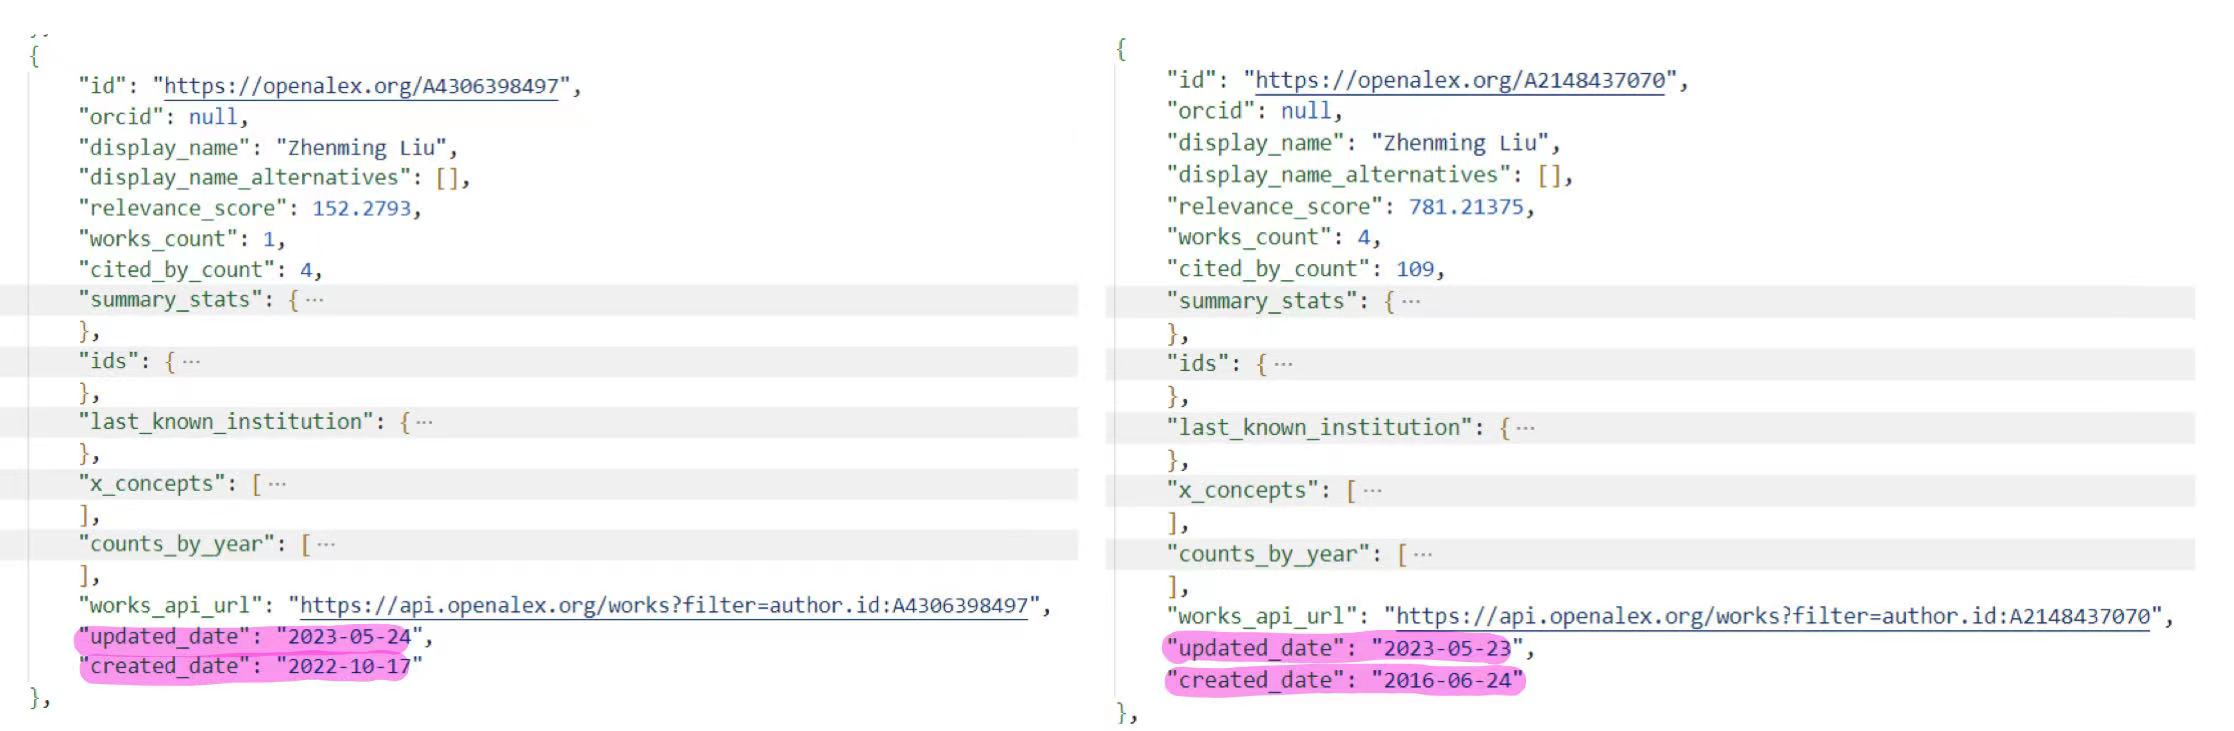
\includegraphics[width=1\textwidth]{./figs/multiple_records.jpg}
  \caption{Same Person With Multiple Records}
  \label{multiple_records}
\end{figure}


\subsection{Google Scholar}
\hspace{0.5cm} Another great academic source is google scholar. It does not have multiple records for the same author and the publications of one author can be found at the author profile page. However, it does not provide an official api. Thus, the only way to fetch author profiles is web scraping. There are several existing ways to do web scraping. The first one is through Serpapi. (\url{https://serpapi.com/google-scholar-api}) It is a paid api that allows user to customize search query, pagination option or some advanced filter options. The second one is a github project: scrape-google-scholar-py.(\url{https://github.com/dimitryzub/scrape-google-scholar-py}) It would simply scrape the searching page and return a classified json result. However, after I tried it to process more than 200 authors, it's blocked by google scholar. Maybe I need to use some customized proxies. The third one is the scholarly python library. (\url{https://scholarly.readthedocs.io/en/stable/quickstart.html}) It's able to solve the CAPTCHA issue to prevent blocking from google scholar, but it still has a everyday using limit. I use scholarly as the final method.
\begin{enumerate}
  \item \textbf{Approach: } Since google scholar supports fuzzy search, for example, you can still get Alman Josh's profile if you search Josh Alman or Alman J. Thus the name aliasing process can be simplified. For John Smith K, I would search for John Smith K, Jhon Smith, Jhon and Smith. Then my search query is name + affiliation. I noticed that google scholar also has email field, so if the name + affiliation pattern does not work, I would try searching name + email.
  \item \textbf{Result and Issue: } I searched a total 500 CS faculties in google scholar and get 459 results. Obviously, it has a lower missing rate than OpenAlex. And google scholar ensures that there is no multiple results for same author and affiliation. However, there are still about 8.2\% authors not found. One possible reason is that Google Scholar allows authors to define their own affiliation names, resulting in lack of consistency. 
\end{enumerate}

\subsection{Combined Result}
\hspace{0.5cm} Then I consider to combine the searching result for both OpenAlex and Google Scholar. I use Google Scholar as a primary searching source. If the author is not found in Google Scholar, I would try to search him/her in OpenAlex. After doing this, among 500 CS faculties, there are only 26 authors not found. I manually check their names and find that most of them are not exist in both datasources. Finally, I append author's Google Scholar id or OpenAlex id to the csv file.
\end{document}
